The point  dividing the line AB in the ratio $m:n$ is given by
\begin{align}
	\vec{P} &=\frac{m \vec{B} + n \vec{A}}{m + n}
\label{1/15eq5}
\end{align}
Let $\vec{A}=\myvec{1\\3}, \vec{B}=\myvec{2\\7}, {m}=3, {n}=4$\\
From \eqref{1/15eq5}
\begin{align}
&=\frac{3\myvec{2\\7}+4\myvec{1\\3}}{3 + 4}\\
&=\frac{\myvec{6\\21}+\myvec{4\\12}}{7}\\
&=\frac{\myvec{10\\33}}{7}\\
&=\myvec{\frac{10}{7}\\\frac{33}{7}}
\end{align}

\begin{figure}[!ht]
	\centering 
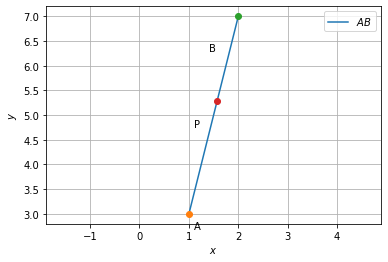
\includegraphics[width=\columnwidth]{solutions/1/15/assignment3.png}
\caption{}
\label{1/15fig:Dividing Line}
\end{figure}
